\chapter{研究方法}


在智能交通中,多目标跟踪技术尤为重要,它时交通流检测、智能驾辅以及交通事件预警等功能的关键性技术之一。本文就是想要改进已有的多目标跟踪模型,并且在仿真实验中进行实验验证从而提高跟踪算法的精度与鲁棒性。


\section{数据收集与预处理}



\subsection{基于仿真场景Town10的交通场景视频收集}





为了获取用于训练和测试的有效数据,我在CARLA仿真平台的 Town10 场景中进行数据采集。基于UE4的强大图形引擎,CARLA能创建高度逼真的城市环境,包括建筑、道路、交通标志、行人和车辆等,支持多种天气和光照条件模拟。

Carla最优势的就是,在CarlaUE4中自带的场景地图中模拟实验,他一不需要购买大量硬件设备和各种高端的传感器;二是他可以模拟各种极端下的危险场景跟极端情况,避免真实测试中可能发生的事故;三是因为它可以精确模拟同一个环境同一个场景下的实验,方便本设计后续去对比。因为他的低成本和方便度,本设计选择了Carla。

如图\ref{fig:p39}所示,Town10 是一个复杂的道路交道区域,具有不同类型的路面、 交通标牌、交通灯和其他各种交通工具以及行人这些活动物体。利用该场景执行仿真脚本后我们可以得到高分辨率的道路交通视频数据,并且获得目标的实际位置信息(真值)。


\begin{figure}[htbp] % 可以是h(here),t(top),b(bottom),p(page of floats)
	\centering
	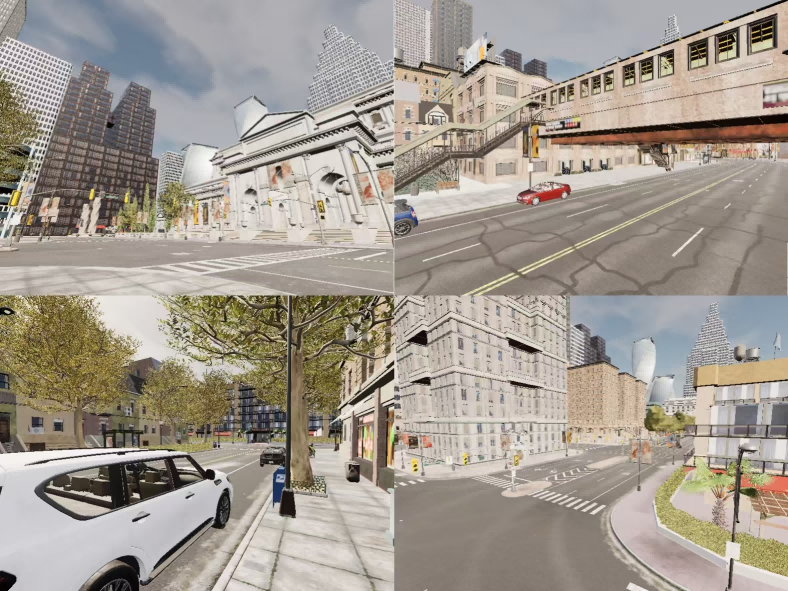
\includegraphics[width=1\textwidth]{p39} % 假设图片文件名为car.pdf或car.png等,位于当前工作目录
	\caption{仿真场景Town10} % 图片标题
	\label{fig:p39} % 用于引用的标签
\end{figure}





\subsubsection{仿真环境搭建}

CARLA仿真平台的安装:采用CARLA-0.9.15版本,保证其能支持多传感器输出和高精度的交通仿真实验。

搭建仿真环境:选用Town10 环境,调整不同的天气状况,时间以及车流,来实现现实生活中丰富的交通环境。

传感器设置:在模拟汽车上布置多传感器,RGB  camera、LiDAR 和毫米波雷达来获得多源信息。

\subsubsection{视频数据收集}

执行仿真脚本:通过 python 脚本来对Carla场景Town10地图里面的仿真汽车进行行驶路线的操控,并且录制摄像头的视频流。本项目中采用的是 traffic twin 的项目中的 Drive.py 文件,在其中改变参数选用不同的控制器、传感器。在开展项目期间,本项目得先搞定数据采集这关键的一步。所以就得依靠 Carla 仿真平台里 Town10 这张地图。通过本设计开发的python 脚本运行,把收集到的安排设计好的汽车行驶路线用摄像头雷达去检测,然后让它复现出收集到的安排设计好的汽车行驶路线。通过这一整套操作,就能拿到可视化数据跟踪收集的结果,为后续的研究打下坚实的基础。

数据存储:将采集到的视频数据存为序列化的文件格式。我们在此项目中是在 Town10 环境下运行了500秒,通过设计的python脚本把每帧抓取出来,一帧就是一张图片。最后将它们保存在同一个文件夹中以进行下一步处理。



\subsection{从模拟器中获取Ground Truth数据}

要想验证跟踪算法的效果,首先必须获得目标的真实运动轨迹,就是Ground Truth。而 CARLA模拟平台他可以提供目标的具体细节,位置,速度,方向等关键参数都很准确。Ground Truth 为设计思路提供了一个精准的参照系,使得设计过程之中能够清晰地看到算法的优劣。


\subsubsection{Ground Truth数据提取}

传感器数据同步:传感器数据和目标真实状态信息在仿真中同步采集。通过CARLA的API能获取每个目标每一帧的精准坐标、速度及朝向,如图\ref{fig:p35}。

数据规范化:将 Ground Truth 数据规范化为结构化的文件形式(CSV或者JSON文件类型),这一举措的主要目的是便于和视频数据进行对齐及处理。可将每一帧中目标的位置、速度、朝向等关键信息存储为一行数据。这样操作就可以让实验设计确保数据的一致性和完整性,还便于本设计在接下来的日子中去读取,处理分析和训练。



\begin{figure}[htbp] % 可以是h(here),t(top),b(bottom),p(page of floats)
	\centering
	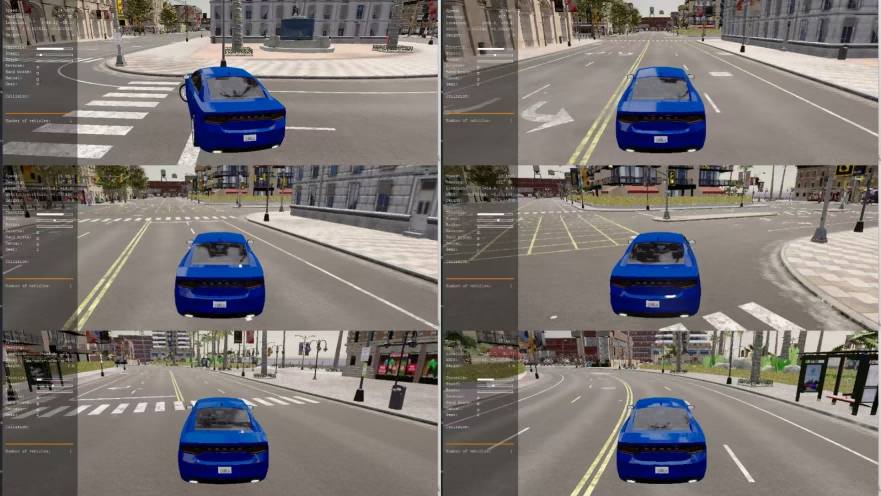
\includegraphics[width=1\textwidth]{p35} % 假设图片文件名为car.pdf或car.png等,位于当前工作目录
	\caption{数据提取} % 图片标题
	\label{fig:p35} % 用于引用的标签
\end{figure}



\subsubsection{数据预处理}

数据清洗:去除噪声数据和异常值,确保数据的准确性和一致性。

数据标注:给视频数据打标签,标出每个目标的类别(例如车、人)及 bounding box 位置。可以采用自动化的标注软件或者人工标注。

数据扩增:利用数据扩增方法(旋转,放大,剪切)来增加数据量,增强模型的泛化性能。








\section{处理轨迹数据}

\subsection{收集轨迹坐标数据}

Town10 场景,执行collect intersection camera lidar.py收集多目标跟踪的测试数据,其中每个十字路口中心有 1 个激光雷达,雷达周围布局有 6 个 RGB 相机,收集每一帧的 6 个视角的场景图像和点云数据,存放在./multi obj track 中,在 collect intersection camera lidar.py 脚本中,设置DATA MUN = 500,表示收集 500 帧的 6 个视角的场景图像和点云数据如图\ref{fig:p41},方便后续操作。



\begin{figure}[htbp] % 可以是h(here),t(top),b(bottom),p(page of floats)
	\centering
	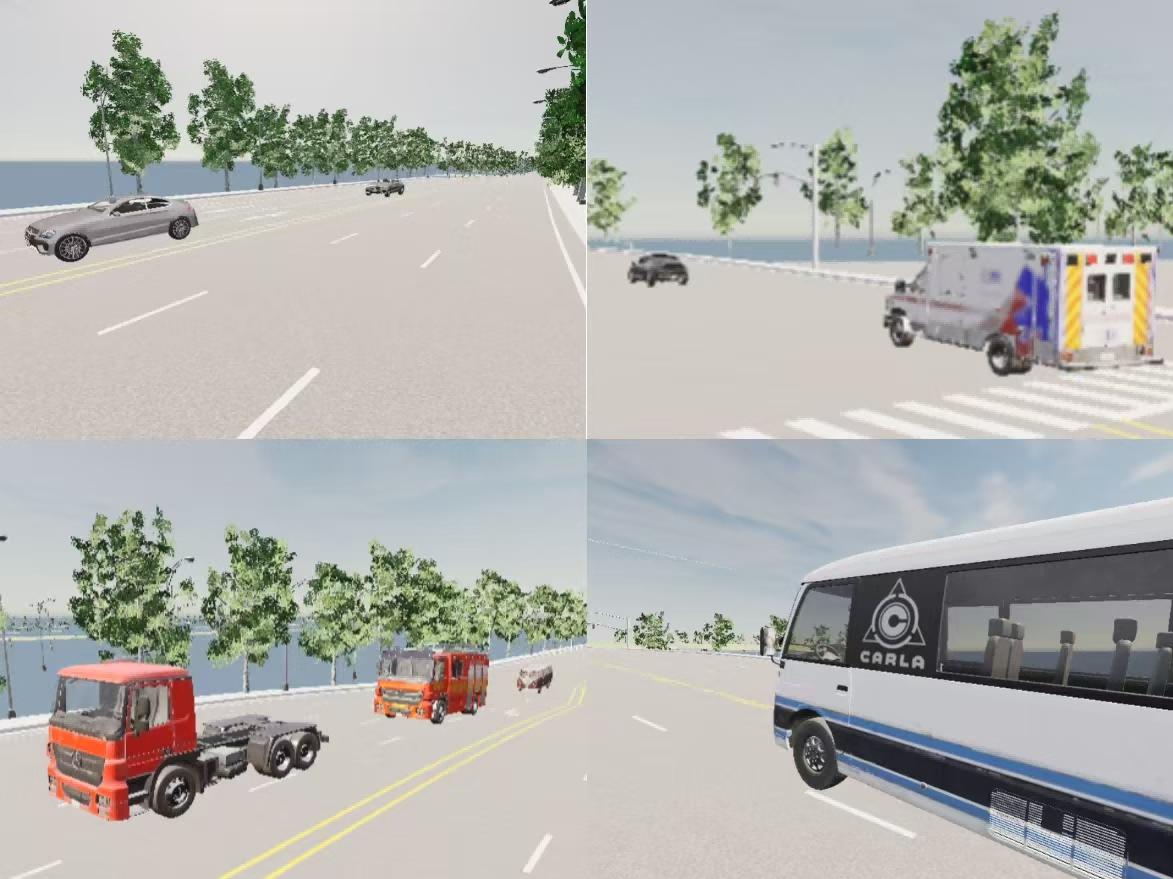
\includegraphics[width=1\textwidth]{p41} % 假设图片文件名为car.pdf或car.png等,位于当前工作目录
	\caption{收集轨迹坐标数据中} % 图片标题
	\label{fig:p41} % 用于引用的标签
\end{figure}






\subsection{轨迹坐标数据预处理}

detect3DBoundingBox.m 这个程序是用来在点云数据里找车并给它们打上 3D 标签 的。首先, 它会从指定的地方加载提前训练好的 PointPillars 检测模型。接着, 它会获取 某个文件夹里所有的.mat 文件。对每个文件, 它会先检查有没有有效的点云数据。要是 有,就提取出来并整理成点云对象。之后, 用检测模型来找目标,得到边界框、置信度 和标签,并把这些结果显示出来,最后再存回到原来的文件里。
detect2DBoundingBox.m 这个程序是用来在图片里找车并给它们打上 2D 标签的,这 里直接用了预训练好的 YOLOv4 模型。先初始化 YOLOv4 检测器,然后获取指定文件 夹里的所有.mat 文件。对每个文件检查有没有 datalog 变量,如果有,就一个一个看相机数据并读取图片。用 YOLOv4 检测器找目标,不过会把“traffic light”标签的检测结 果过滤掉。最后把有用的检测结果存回原始文件。



\subsection{获取转化轨迹坐标数据}

multiObjectTracking.m 可视化跟踪的车辆。先进行路径配置与文件加载,初始化显 示与轨迹对象;然后在数据帧处理循环中,依次进行数据加载与时间戳检查、提取检测 数据、检测结果融合、目标跟踪、结果可视化、轨迹更新与保存; 最后将完整轨迹数据 保存至指定文件夹以便后续评估与分析,输出 trackedData.mat。

获取的轨迹是相对于自车的坐标,然而本次设计假设自车是静止在路口中间(实际 不存在),雷达和相机都附着在自车上,也就是说与自车存在一个相对位置,示例中雷达 与车辆的相对位置是 [0,0,0],但本项目中雷达是高出一定的距离。convertTrackToCarla- Coordinate.m 将坐标转换成 CARLA 场景中的轨迹,使用的是相对于自车的,因此 (x,y) 是正确的。

\subsection{轨迹坐标再识别}

首先在次课题设计的是先收集车辆再识别数据集,有了许多数据之后,为了设计后续更好地去训练以及设计最终更好地一个给大众和评委老师展示地效果,还需要在经过数据裁剪(2D 标签进行裁剪)之后,再次训练测试。



\section{轨迹预测分析}



\subsection{现有检测跟踪模型的分析}


而在智能交通中,多目标跟踪主要完成两个任务,目标检测以及数据关联。目前主流的方法有两种,一种是检测基础上的跟踪 (Track-by-Detection), 另外一种是端对端的跟踪(End-to-End Tracking)。检测基础上的追踪顾名思义,它就是采用目标检测的方法先从每一幅图像中找出所有目标的可能性,之后再用数据关联来将这些目标候选和之前的目标轨迹对应起来,就好像先寻找人并发现他的存在,在跟踪人的行动一般。而端到端的跟踪更复杂一些,它采用深度学习的方法将目标检测与数据关联结合到一起,一整个视频输入,目标的路径就出来了。


\subsubsection{基于检测的跟踪模型}

为了寻找目标位置,常使用的有YOLO、Faster R-CNN、SSD等检测算法,它们在速度与准确度方面有着不同的表现。例如YOLO算法,速度快得惊人,可以实现实时性输出结果,但是准确率方面相对较低;而Faster R-CNN更重视准确率,输出结果细粒 度强,可是运算繁琐,速度相对较慢。


\subsubsection{端到端的跟踪模型}


在深度学习模型设计上,端到端跟踪结构常常将卷积神经网络(CNN)与循环神经网络(RNN)相联合。就拿经典算法来说,SORT 算法将卡尔曼滤波与匈牙利算法相结实时追踪框架。DeepSORT算法更强,它在sort基础上引入深度学习的特征提取模块,采用外观建模提升跟踪稳定性。

但是端到端跟踪模型比较复杂,训练时会消耗大量的算力和大尺度的标签数据集作为其支持。然而智慧交通对模型实时性要求又比较高,在应用过程中就需要对模型进行设计优化。优化的方式主要有加入轻量级的网络结构,减少其所需要的计算量;或者是模型本身采用模型剪枝、量化等压缩方式来加快推理速度。这样一来,模型便既可以在性能的基础上达到实时性的需求。


\subsection{模型优化策略与方法}

\subsubsection{模型结构优化}

轻量化网络结构:使用轻量化的卷积神经网络(MobileNet、ShuffleNet)作为目标检测单元,降低计算负担,增强实时能力。

特征融合:利用多种类型信息(RGB图像、激光雷达点云等如图\ref{fig:p40})进行特征融合提升了目标检测与跟踪的精度。可以采用注意力机制及多尺度特征融合方法,提升了复杂场景下模型的效果。

模型压缩加速:基于剪枝、量化、知识蒸馏等方法对预训练模型进行压缩加速,减少模型存储和计算开销。





\begin{figure}[htbp] % 可以是h(here),t(top),b(bottom),p(page of floats)
	\centering
	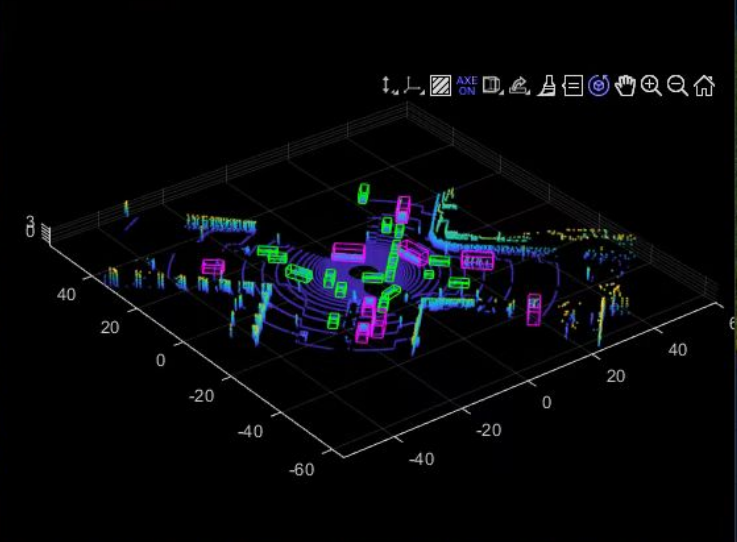
\includegraphics[width=1\textwidth]{p40} % 假设图片文件名为car.pdf或car.png等,位于当前工作目录
	\caption{激光雷达检测} % 图片标题
	\label{fig:p40} % 用于引用的标签
\end{figure}







\subsubsection{数据关联优化}

优化跟踪关联算法:增加深度学习特征提取,例如用ResNet或者Inception网络提取目标的外观信息,与卡曼滤波、匈牙利算法相结合进行跟踪关联,并且提升了关联正确性和稳定性。

多目标关联:利用图神经网络(GNN)或者注意力机制,对多个对象间的关系进行建模,提升在复杂场景的跟踪效果。

\subsubsection{训练策略优化}

数据扩增及正则化:利用数据扩增技术(随机翻转、缩放、裁剪)增加数据集,使得模型具有更好的泛化能力。另外,使用正则化技术(Dropout,L2正则化)来避免模型过拟合。

迁移学习、微调:以在大规模数据集上训练好的通用模型为基础,借助迁移学习和微调技术,迅速针对特定的交通环境和目标对象进行调整。


\subsection{性能指标的选择与定义}

为了综合评价优化后的多目标跟踪模型性能,选择了下面的10项性能度量并定义了计算方式:

\subsubsection{目标检测指标}
准确率(Precision):检测到的目标中实际为正样本的比例,计算公式为:
\[\text{Precision} = \frac{\text{TP}}{\text{TP} + \text{FP}}\]
其中,TP表示真正例,FP表示假正例。

召回率(Recall):实际为正样本的目标中被检测到的比例,计算公式为:
\[\text{Recall} = \frac{\text{TP}}{\text{TP} + \text{FN}}\]
其中,FN表示假负例。

平均精度(mAP):综合考虑准确率和召回率的指标,计算公式为:
\[\text{mAP} = \frac{1}{N} \sum_{i=1}^{N} \text{AP}_i\]
其中,N表示类别数量,AP表示每个类别的平均精度。

\subsubsection{数据关联指标}
轨迹精度(Trajectory Precision):跟踪轨迹中正确匹配的目标比例,计算公式为:
\[\text{Trajectory Precision} = \frac{\text{正确匹配的轨迹点数量}}{\text{总轨迹点数量}}\]

轨迹召回率(Trajectory Recall):GroundTruth轨迹中被正确跟踪的比例,计算公式为:
\[\text{Trajectory Recall} = \frac{\text{正确跟踪的轨迹点数量}}{\text{Ground Truth轨迹点数量}}\]

\subsubsection{跟踪性能指标}

跟踪成功率(Tracking Success Rate):在所有测试序列中,跟踪成功的目标比例,计算公式为:
\[\text{Tracking Success Rate} = \frac{\text{跟踪成功的目标数量}}{\text{总目标数量}}\]

平均跟踪误差(Mean Tracking Error):跟踪轨迹与Ground Truth轨迹之间的平均误差,计算公式为:
\[\text{Mean Tracking Error} = \frac{1}{N} \sum_{i=1}^{N} \text{Error}_i\]
其中,N表示轨迹点数量,Error表示每个轨迹点的误差。




拥有以上的这些指标后,就可以对多目标跟踪算法的性能进行系统而全面的评估,为算法的优化和改进提供明确的方向与依据。







